\subsubsection{Real photons}
%Contributed by Klaus Reygers, Ana Marin, Dmitri Peresunko

Recently ALICE has measured direct photon spectrum in three centrality classes in Pb--Pb collisions at $\sqrt{s_{\rm NN}}=2.76$ TeV, see Fig.\ \ref{fig:RealPhotonsRg}, left. The measurement combines results of Photon Conversion Method (PCM) and of PHOS spectrometer. In central collisions at low \pT<3-4 GeV/$c$ an excess with respect to prompt photon predictions is observed that is attributed to thermal photon emission from the QGP. For the most central 0-20\% centrality the low \pT \ excess is of the order of 10-15\%, while the total uncertainty of the order of 6\%. A signal of direct photons was found in central collisions, but on the level ~2 sigma, while in mid-central and especially in peripheral situation is even worse. On the other hand peripheral collisions are important since there one can estimate and restrict contribution from prompt direct photons.  

%-----------------------------------------------------------------------%
\begin{figure}[hbt]
\centering
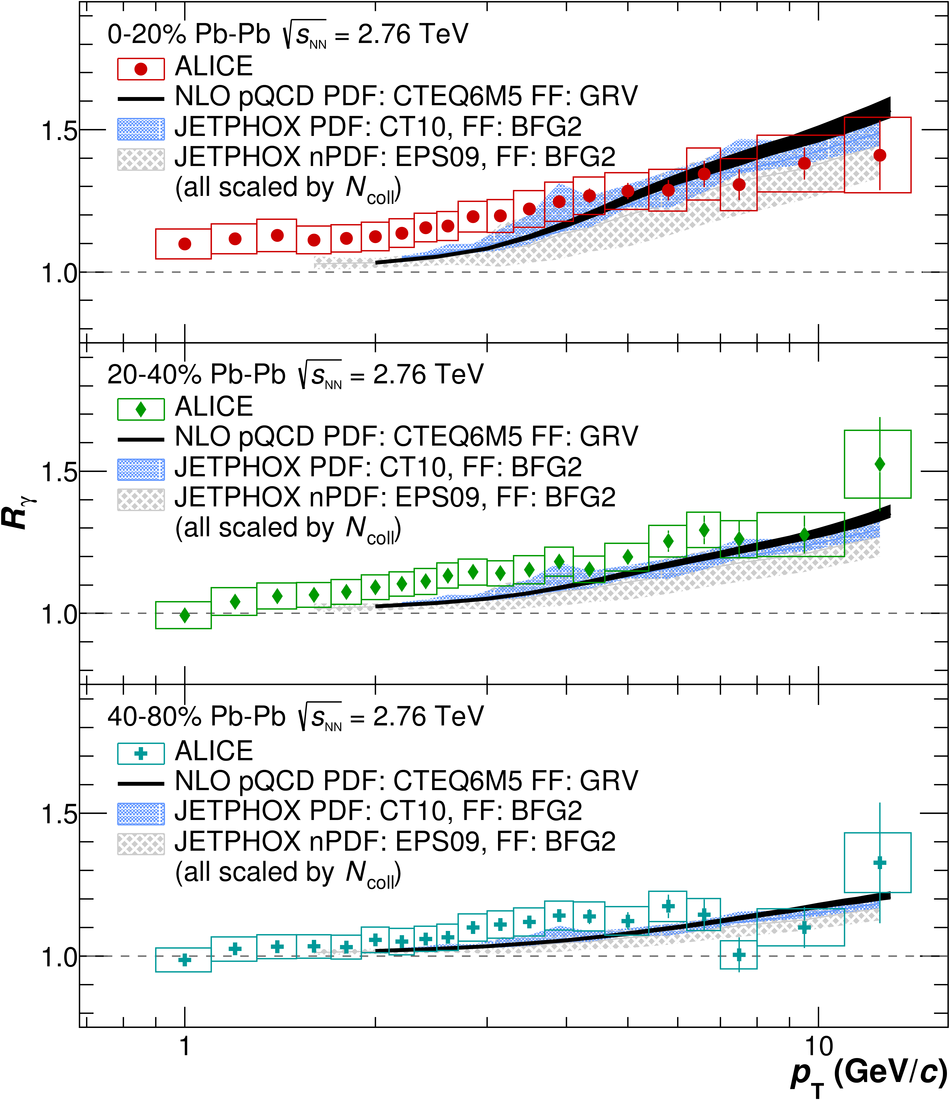
\includegraphics[width=0.46\textwidth]{\main/thermalradiation/figs/RgammaRun1}
\hfill
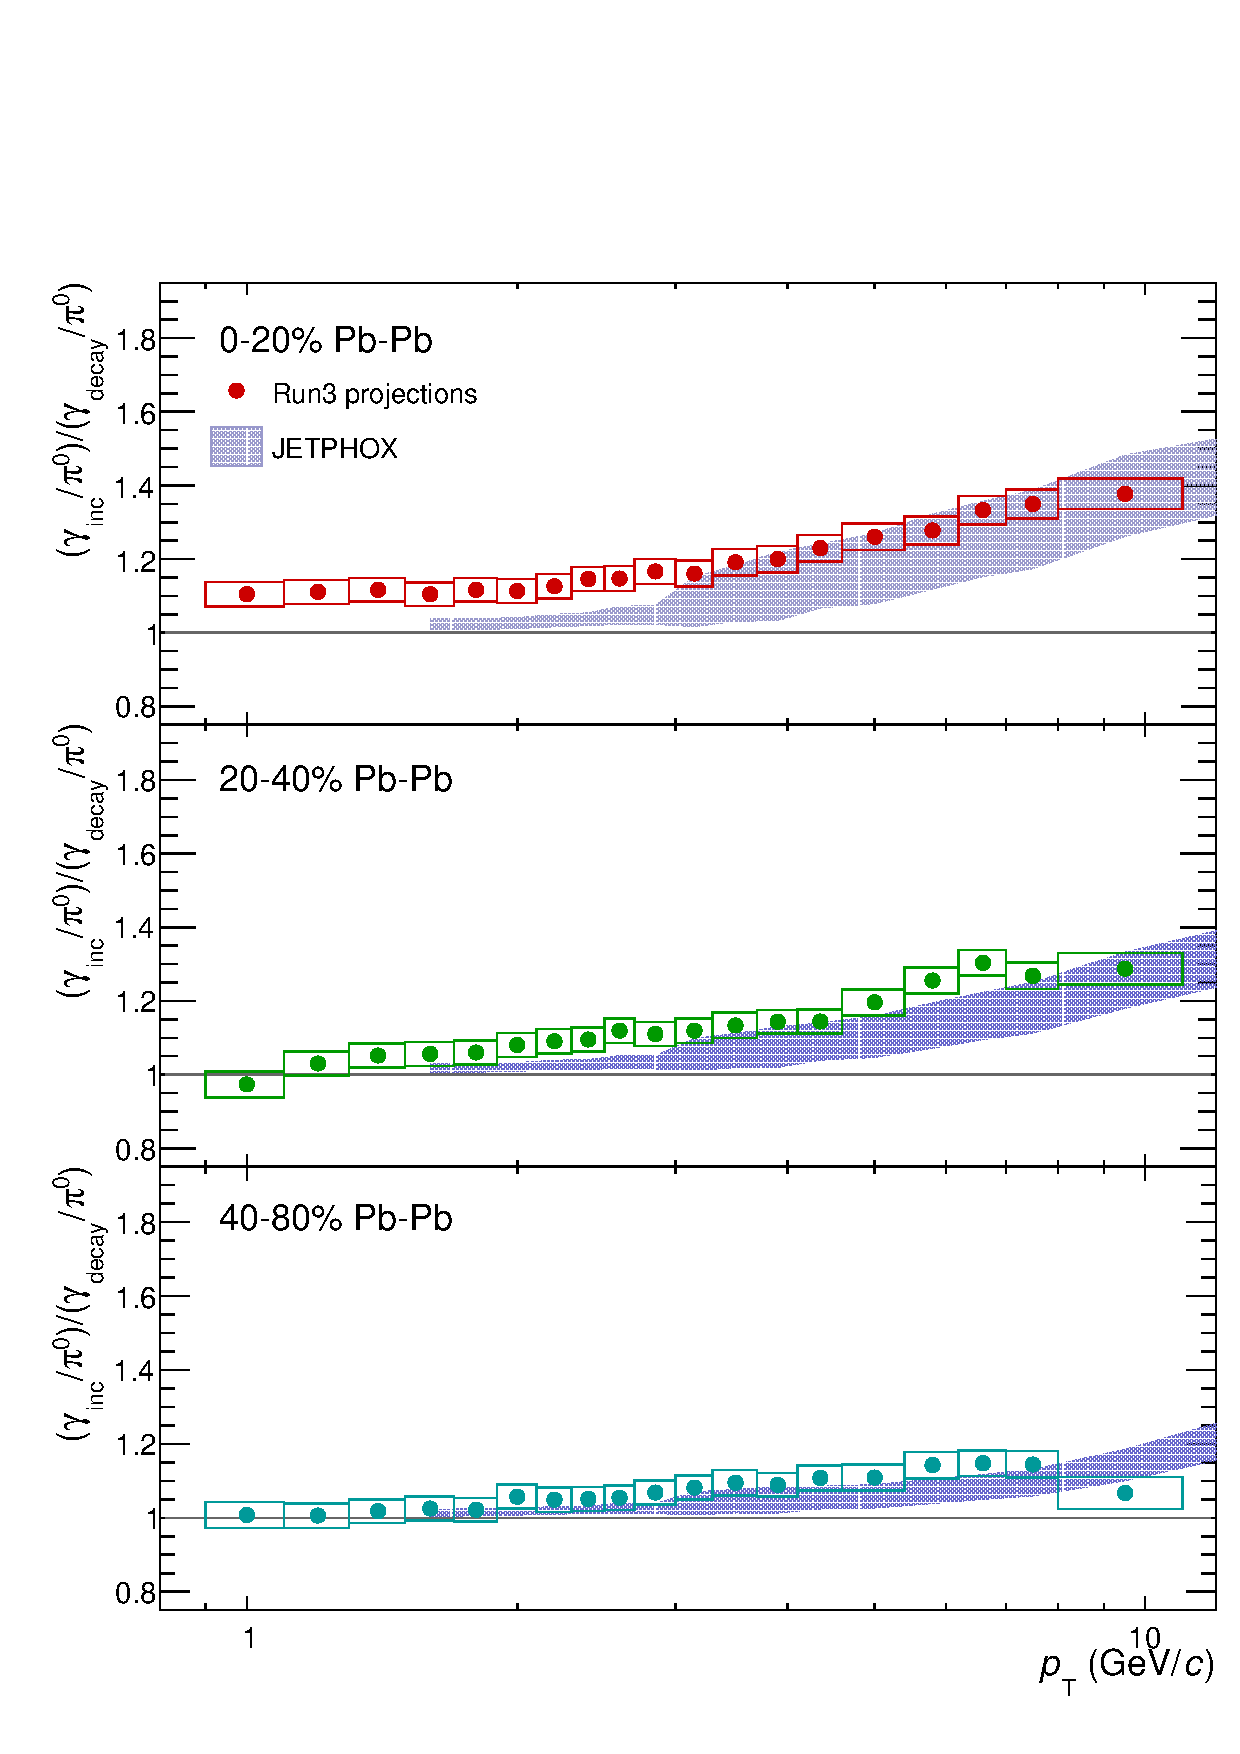
\includegraphics[width=0.425\textwidth]{\main/thermalradiation/figs/ReducedRg.pdf}
\caption{$R_{\gamma}$ measured (left) and $R_{\gamma}$ projected.}
\label{fig:RealPhotonsRg}
\end{figure}
%-----------------------------------------------------------------------%

Let us consider how one can improve accuracy of our measurement. We split uncertainties into 3 classes: those which can be improved with increase of statistics (statistical uncertainties, uncertainties related to $\pi^0$ spectrum extraction, $\eta/\pi^0$ ratio); uncertainties which can be reduced using new techniques and some special methods (material budget estimate - with calibrated material analysis, energy scale in calorimeters with new hybrid $\pi^0$ methods); and uncertainties related to the properties of the detector which can not be improved (hadron contamination in calorimeters, electron identification in conversion method etc.). To estimate improvement of uncertainties we assumed that available statistics will increase by factor 100. 
The main contributor to the systematic uncertainties at 
low \pT\  for PCM is the material budget uncertainty with 4.5\%. 
The major improvement foreseen for Run-3 is the installation of two 1~\ mm tungsten wires with well known material thickness parallel to the beam direction in the new ITS. The wires will be positioned 
between layers 2-3 and 4-5 at R = 4-14 cm and R = 30.9 cm, being inclined the most inner one. 
In order to do so, a method to calibrate the material budget is proposed. 
The yield of $\gamma$ conversions with production in the wire would be used to calibrate the product 
of the photon flux times $\gamma \rightarrow e^+e^-$  reconstruction efficiency.
This product would then be used to precisely determine the material thickness in the rest of the ITS (assuming phi-independent photon flux and taking the radial dependence of the reconstruction efficiency from simulation).


The method proposed to calibrate the complete ITS material thickness is based on weights calculated as  a double ratio of reconstructed  $\gamma$ conversions in a generic radial bin to the number of reconstructed conversions in the calibrated material in Data to the same ratio in Monte Carlo. 
The weights are calculated as: 
\begin{equation}
\omega_i= \left .{\left(\frac{N_\gamma^{rec}(r_i)}{N_\gamma^{rec}(r_{gas})}\right)^{DATA}} \right /{\left(\frac{N_\gamma^{rec}(r_i)}{N_\gamma^{rec}(r_{gas})}\right)^{MC}} ,
\end{equation}
Weights different from 1, correspond to deviating material in the simulation.
These weights are then used to scale the reconstruction efficiency in each radial bin of the detector.
This procedure is being implemented for Run-2 data using the TPC gas as calibration material. First results
show that a systematic uncertainty of 1.8\% can be achieved.

{\bf Compare of different predictions Rg, with expected uncertainties: can we distinguish theories? Can we establish direct (thermal) photon measurements with 5 sigma? (Ana collect predictions and make Rg for 5 TeV, Cocktail: 5 TeV prelim pi0+eta/pi0 from 2.76)

To which extend should we reduce sys/stat uncertainties to reach 5 sigma? Use our code.
}

Observation of the collective flow of final hadrons was one of the most important findings in the area of heavy ion collisions.
Collective flow is the azimuthal asymmetry in particle production, common for all soft particles in the collision. 
It is interpreted as a collective expansion of initially spatially asymmetric hot matter. This initial deformation is the result of partial overlap of colliding nuclei in non-central collisions.  Transforming the initial geometric asymmetry into the asymmetry of momentum distribution of final particles requires strong interaction between particles of the matter, therefore hydrodynamic-like models provide very good description of this effect. 
Direct photons do not interact with hot matter and deliver information about the collective  flow at the moment of their emission. As hydrodynamic models predict, photons emitted at the initial stage by hot quark-gluon matter carry very small collective flow since it is not developed yet at this stage. In contrast, direct photons emitted at the latest stage of hadron gas expansion carry much larger collective flow, similar to one of final hadrons. 
Averaging over the whole history of the collision leads to the prediction of direct photon flow considerably smaller than one of final hadrons. 
However, the first measurements of direct photon elliptic flow $v_{2}$ performed by PHENIX experiment \cite{Adare:2011zr}, demonstrated that the direct photon flow is comparable with one of final hadrons and much larger than one predicted by hydrodynamic models. 

ALICE performed measurements of the direct photon elliptic flow in Pb--Pb collisions at $\sqrt{s_{NN}}=2.76$ TeV for the two centrality classes, 0--20\% and 20--40\%, see Fig.~\ref{fig:RealPhotonsV2dir}.
We compare the measured direct photon elliptic flow $v_2^{\gamma,\rm dir}$ to the estimated decay photon elliptic flow $v_2^{\gamma,\rm dec}$, marked as cocktail, and to the predictions of several theoretical models. We find that, similar to RHIC measurements, the direct and decay photon elliptic flow are very close. 
We compare our measurements to state-of-the-art hydrodynamic model calculations \cite{Gale:2014dfa,Chatterjee:2017akg} and the transport model \cite{Linnyk:2015tha}. The measured direct photon elliptic flow is systematically higher than theoretical predictions, but because of the large uncertainties they are statistically consistent. As one can see, uncertainties are relatively large and one can not presently exclude neither of theoretical calculations. 
{\bf We estimated v2dir with updated Rg uncertainties}

%-----------------------------------------------------------------------%
\begin{figure}[htb]
\centering
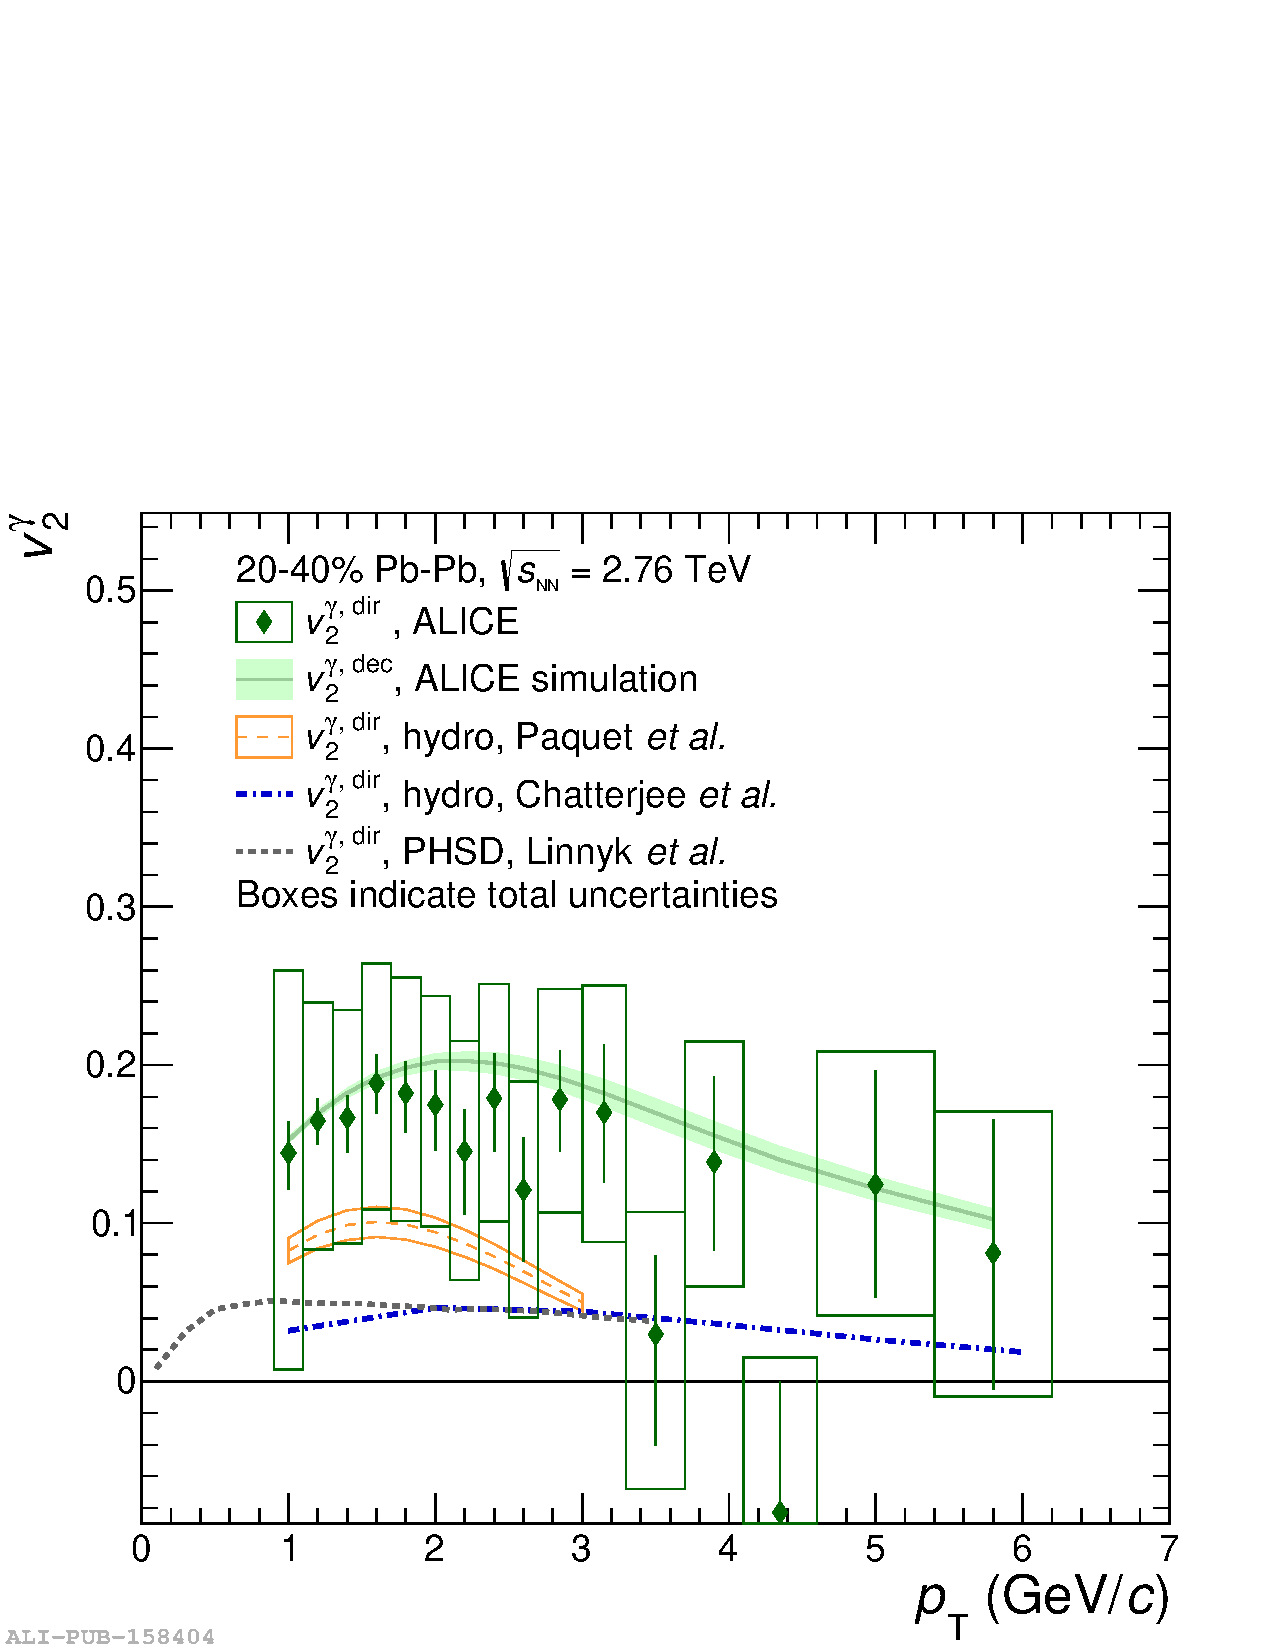
\includegraphics[width=0.45\textwidth]{\main/thermalradiation/figs/2018-May-11-2040_v2dir_combined_theory}
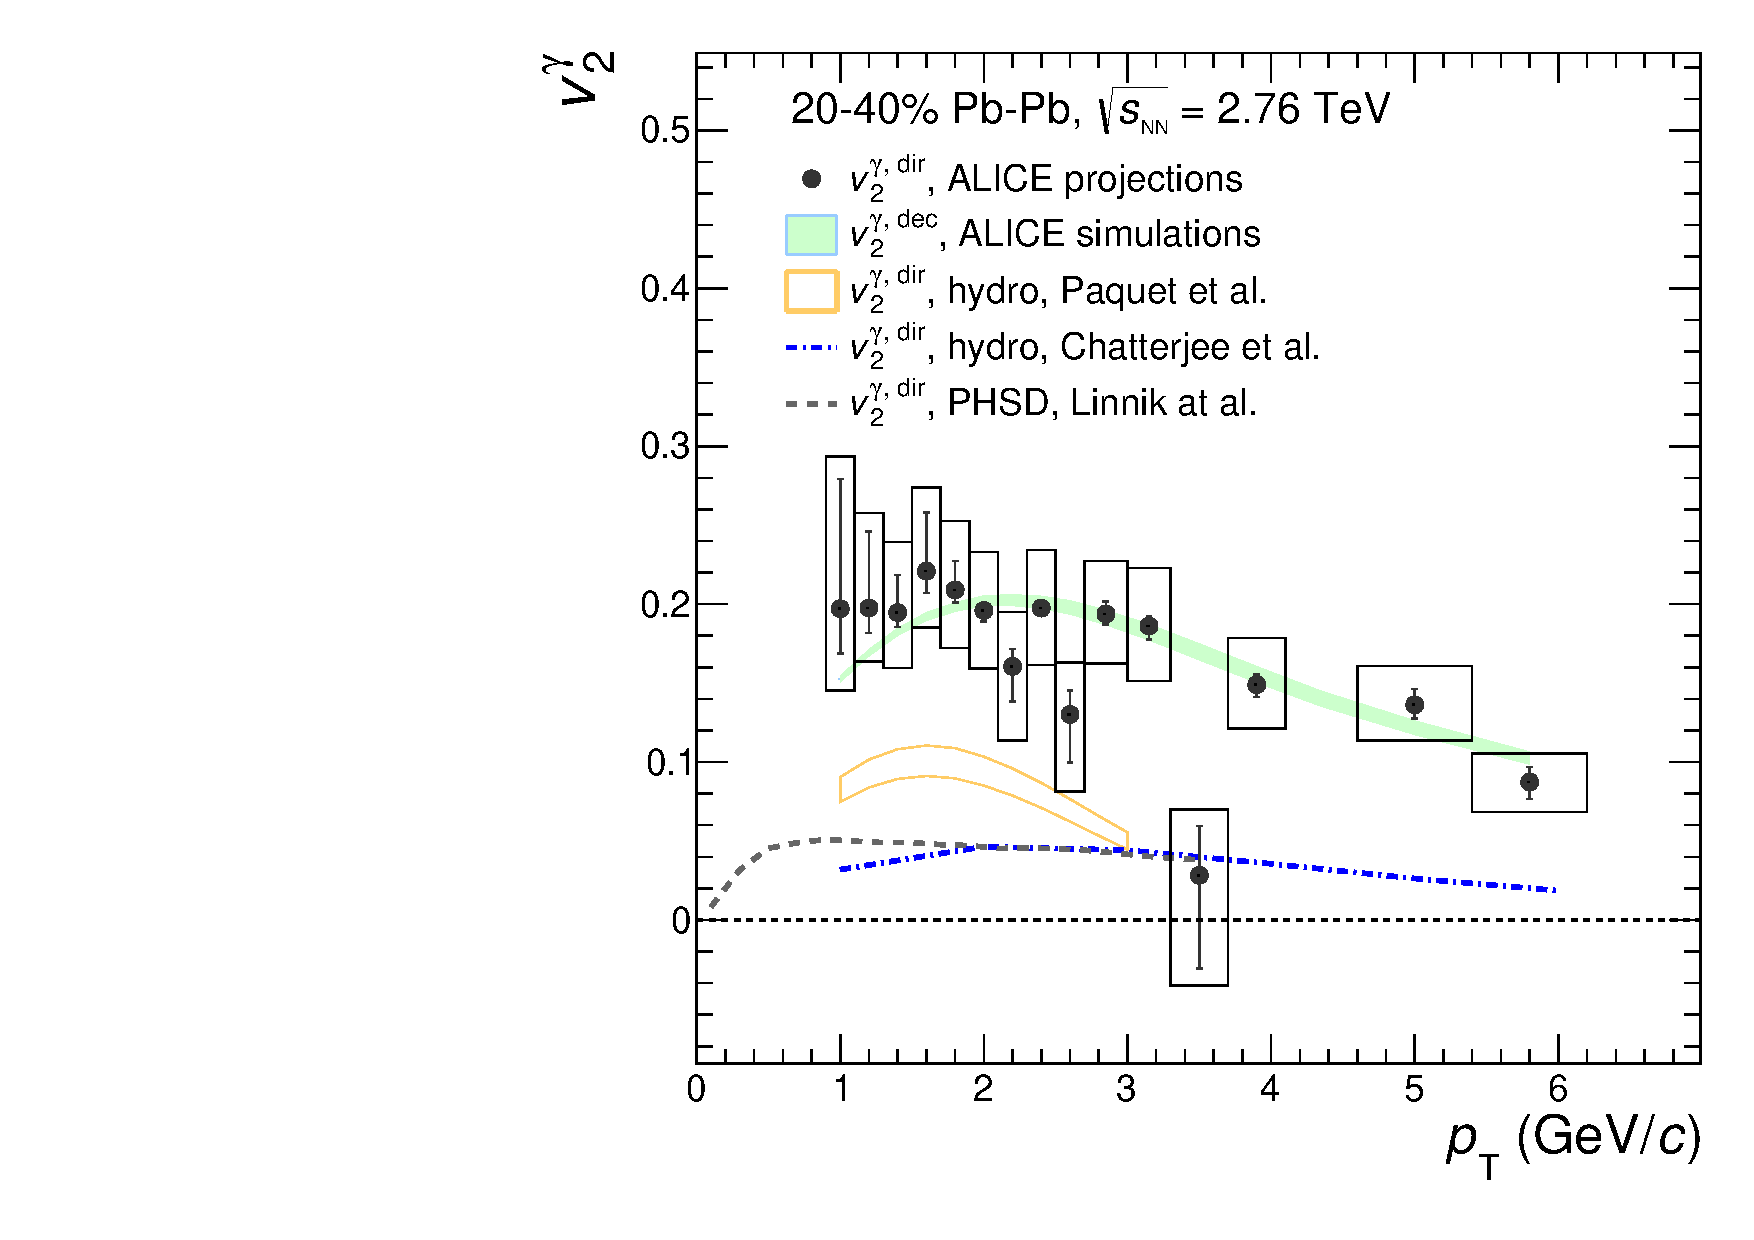
\includegraphics[width=0.42\textwidth]{\main/thermalradiation/figs/ProjectionV2.pdf}
\caption{Direct photon flow in mid-central collisions. Left: direct photon collective flow measured in Pb-Pb collisions compared to decay photon flow and several theoretical predictions. Right: expected accuracy in Run3. }
\label{fig:RealPhotonsV2dir}
\end{figure}
%-----------------------------------------------------------------------%




\begin{itemize}
\item First measurement at LHC from soft exponential component of photon pT spectrum (ALICE, Phys.Lett. B754 (2016) 235): T ~ 300 MeV (effective temperature averaged over system evolution)
\item "Photon puzzle"
\item Projections for Run3/4 in preparation: reduce systematic error (material budget uncertainty)
\end{itemize}
